\chapter*{Введение}                         % Заголовок
\addcontentsline{toc}{chapter}{Введение}    % Добавляем его в оглавление

\paragraph*{Актуальность темы.}
%
В современном мире существует множество различных приложений, в которых возникают задачи большой размерности.
Особенно это актуально в контексте задач синтеза и верификации дискретных управляющих (ДУ) систем, таких как конечные автоматы и логические схемы.
Основная проблема заключается в синтезе ДУ-моделей с требуемыми свойствами, которые характеризуются комбинаторной природой и могут быть построены различными способами.
Алгоритмы управления, задаваемые с помощью конечных автоматов или логических схем, могут быть синтезированы как по заданным примерам поведения, так и по формальной спецификации, например, в случае описания свойств конечно-автоматных моделей \--- на языке темпоральной логики.

% TODO: описать NP-полноту задач синтеза и верификации, привести ссылки

Распространённым подходом к \emph{автоматическому} синтезу и верификации является \emph{сведение} к классическим NP-полным задачам, таким как задача выполнимости булевой формулы (Boolean satisfiability problem, SAT), задача максимальной выполнимости (MaxSAT) и задача выполнимости в теориях (Satisfiability Modulo Theory, SMT), с последующим применением так называемых \emph{решателей}, реализующих современные алгоритмы решения этих задач.
Данные задачи являются \enquote{универсальными}, в том смысле что они могут быть использованы для решения широкого класса задач, исключая тем самым необходимость разработки специализированных алгоритмов для каждой конкретной задачи.
Однако все известные алгоритмы решения таких задач имеют экспоненциальную сложность в худшем случае.
Таким образом, актуальной является проблема повышения эффективности комбинаторных алгоритмов в применении к вышеупомянутым задачам синтеза и верификации ДУ-моделей.
% В рамках данной диссертации рассматривается один из подходов к решению этой проблемы \--- \emph{построение декомпозиций булевых формул}, которые кодируют рассматриваемые задачи.
% Это позволит справиться с комбинаторной сложностью и обеспечить более эффективное и точное синтезирование ДУ-моделей с требуемыми свойствами.
% Именно эта задача является центральной в данной диссертации.


\todo{Одна из центральных проблем -- отсутствие априорных оценок времени работы алгоритмов решения задачи SAT. В диссере предлагаются и развиваются методы/алгоритмы, которые позволяют строить такие оценки. Для этого используются специальные декомпозиционные представления булевых формул.}
\todo{Идеи построения декомпозиций уже выдвигались, но они обладают меньшей точностью. Наши методы декомпозиции учитывают особенности исходной задачи, которую мы решает с помощью сведения к SAT, например особенности задачи синтеза конечно-автоматных моделей или задачи проверки эквивалентности логических схем.}


\paragraph*{Цель работы.}
%
Целью данной работы является повышение эффективности работы полных алгоритмов решения задачи SAT в применении к задачам синтеза и верификации ДУ-моделей за счет оригинальных методов и техник декомпозиции булевых формул.


\paragraph*{Задачи работы.}
%
Для~достижения поставленной цели были решены следующие научно-технические задачи:
\begin{enumerate}[beginpenalty=10000]
    \item Разработаны оригинальные алгоритмы кодирования в SAT задач синтеза конечно-автоматных моделей с заданным поведением и свойствами, отличающиеся от существующих добавлением кодирования структуры охранных условий в виде деревье разбора соответствующих формул.
    \item Разработаны оригинальные алгоритмы кодирования в SAT задач синтеза модульных конечно-автоматных моделей с заданным поведением и свойствами, отличающиеся от существующих автоматизированным модульным разбиением.
    \item Разработаны оригинальные методы оценивания декомпозиционной трудности булевых формул, кодирующих задачи синтеза конечно-автоматных моделей и верификации булевых схем, отличающиеся от существующих учётом особенностей исходной задачи, а также низкой дисперсией времени решения подзадач.
    \item \todo{Разработаны новые алгоритмы решения трудных вариантов SAT, использующие понятие вероятностных лазеек (backdoors).}
    \item С применением разработанных алгоритмов решены трудные примеры задач синтеза ДУ-моделей (как конечно-автоматных моделей, так и логических схем).
    \item \todo{Разработан новый SAT решатель, использующий вероятностные лазейки для вывода новой информации при работе с трудными булевыми формулами.}
    \item \todo{Разработана библиотека алгоритмов ... + вычислительные эксперименты.}
\end{enumerate}


\paragraph*{Методы и инструменты исследования.}
%
\todo{переписать}
Теоретическая часть работы использует методологию дискретной математики и математической логики, теории вычислительной сложности,а также теорию эволюционных вычислений.
\todo{Для синтеза конечно-автоматных моделей был использован программный комплекс fbSAT, разработанный в рамках данной диссертации.} \todo{ссылка}
При построении вычислительных задач из области проверки логической эквивалентности схем использовалась программная система Transalg \todo{ссылка}.
Для решения конкретных инстансов задачи SAT использовались различные современные SAT-решатели, находящиеся в открытом доступе, такие как MiniSAT, Glucose, Kissat, Cadical \todo{ссылки}.
В вычислительных экспериментах задействовался вычислительный кластер.


\paragraph*{Основные положения, выносимые на защиту.}
%
\begin{enumerate}[beginpenalty=10000]
    \item Оригинальные алгоритмы кодирования в SAT задач синтеза конечно-автоматных моделей, отличающиеся от существующих добавлением кодирования структуры охранных условий в виде деревье разбора соответствующих формул.

    \item Оригинальные алгоритмы оценивания декомпозиционной трудности булевых формул применительно к задачам верификации логических схем, отличающиеся от существующих учётом особенностей исходной задачи.

    \item Новые алгоритмы решения трудных вариантов SAT, использующие понятие вероятностных лазеек ($\rho$-backdoors).

    % \item Алгоритмы решения трудных вариантов SAT на основе объединения нескольких вероятностных лазеек;

    % \item Семейство алгоритмов, вошедших в состав нового SAT решателя, базирующегося на концепции вероятностных лазеек.
\end{enumerate}


\paragraph*{Научная новизна.}
%
Новыми являются все основные результаты, полученные в диссертации, в том числе:
\begin{enumerate}[beginpenalty=10000]
    \item Новые алгоритмы синтеза конечно-автоматных и модульных конечно-автоматных моделей, основанные на сведении к проблеме булевой выполнимости (SAT).

    \item Новые методы оценивания декомпозиционной трудности булевых формул, кодирующих задачи синтеза ДУ-моделей.

    \item Оригинальные алгоритмы решения трудных инстансов задачи SAT, использующие объединение нескольких вероятностных лазеек.

    \item Решение экстремально трудных задач синтеза ДУ-моделей при помощи разработанных алгоритмов.
\end{enumerate}


\paragraph*{Теоретическая и практическая значимость работы.}
%
Теоретическая значимость диссертации заключается в разработанных в ней концепциях и алгоритмах решения задач синтеза ДУ-моделей и методах построения оценок трудности таких задач.
Практическая значимость диссертации состоит в том, что основные разработанные в ней алгоритмы применимы к индустриальным задачам синтеза и верификации ДУ-моделей, а также в том, что на целом ряде конкретных примеров практическая реализация и апробация разработанных  алгоритмов демонстрируют лучшую эффективность в сравнении с известными подходами.


\paragraph*{Соответствие специальности.}
%
Содержание научно-квалификационной работы охватывает такие направления как: синтез и верификация управляющих систем дискретной природы; разработку проблемно-ориентированных комбинаторных алгоритмов, применимых к автоматическому проектированию и верификации ДУ-моделей; разработку алгоритмов декомпозиции сложных эксземпляров комбинаторных задач; разрработку программных средств для эффективного взаимодействия и SAT-решателями; разработку специализированных SAT-решателей, учитывающих особенности решаемых задач.
Таким образом, можно утверждать, что работа соответствует паспорту специальности 2.3.5 (05.13.11) в пунктах 1 и 3.


\paragraph*{Достоверность научных достижений.}

\todo{TODO}


\paragraph*{Апробация работы.}
%
\todo{TODO} Основные результаты работы докладывались~на: перечисление основных конференций, симпозиумов и~т.\:п.

\todo{ГРАНТЫ:}
\begin{itemize}
    \item Грант РФФИ №19-07-01195 А «Разработка методов машинного
    обучения на основе SAT-решателей для синтеза модульных логических контроллеров киберфизических систем».
    \item Грант №19-37-51066 Научное наставничество «Разработка методов синтеза конечно-автоматных алгоритмов управления для программируемых логических контроллеров в распределенных киберфизических системах».
\end{itemize}


% \paragraph*{Внедрение результатов работы.}


\paragraph*{Публикации.}
%
Список всех публикаций автора по теме диссертации:
%
\begin{refsection}[biblio/own.bib]
\nocite{*}
\printbibliography[
    keyword=own,
    %title={Список всех публикаций автора по теме диссертации},
    %heading=subbibliography,
    heading=none,
    resetnumbers=true
]
\end{refsection}



\paragraph*{Структура и объем диссертации.}
%
Диссертация состоит из~введения,
\formbytotal{totalchapter}{глав}{ы}{}{},
заключения и
\formbytotal{totalappendix}{приложен}{ия}{ий}{ий}.
Полный объём диссертации составляет
\formbytotal{TotPages}{страниц}{у}{ы}{}, включая
\formbytotal{totalcount@figure}{рисун}{ок}{ка}{ков} и
\formbytotal{totalcount@table}{таблиц}{у}{ы}{}.
Список литературы содержит
\formbytotal{citenum}{наименован}{ие}{ия}{ий}.

% \begin{figure}
%     \centering
%     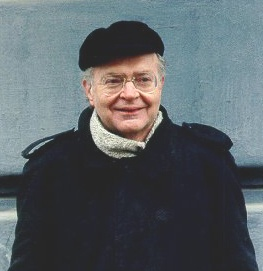
\includegraphics[width=0.6\linewidth]{images/knuth}
%     \caption{Knuth}
%     \label{fig:my_label}
% \end{figure}
